\chapter{Related Work}
According to \cite{zhao2023explainabilitylargelanguagemodels}, the training of \acrshort{llm}s can be categorized into two paradigms, namely \textit{traditional fine-tuning} and \textit{prompting} depending on how they are adapted for downstream tasks (see Figure~\ref{fig:llm_explainability}). 
\\\\
In \textit{traditional fine-tuning}, the \acrlong{llm} is pre-trained on a large corpus of unlabeled text data and further fine-tuned on labeled data tailored to a specific domain and bench-marked accordingly (for example, the GLUE benchmark \cite{wang2019gluemultitaskbenchmarkanalysis}). In the \textit{prompting} paradigm the so-called \textit{prompts} enable the model to behave in a certain way without retraining it, enabling zero-shot, one-shot and few-shot learning without requiring additional training data \cite{brown2020languagemodelsfewshotlearners}. 
\\\\
As stated in section~\ref{sec:xai} and shown in Figure~\ref{fig:llm_explainability}, \textit{Gradient-Based Explanation} is a subcategory of \textit{feature attribution-based explanation}. However, the approach presented in this article falls under \textit{example-based explanation} (or in other words \textit{instance-based explanation}) but also uses a kind of gradient-based solution and therefore \textit{gradient-based explanation} will be briefly described in the next section.

\section{Gradient-Based Explanation}
The importance of each input feature can be evaluated using gradient-based attribution techniques. This is achieved by analyzing the partial derivatives of the output with respect to each input dimension. The magnitude of the derivatives reveals how sensitive the output is to changes in the input. This method can generally be formulated as $s_j=\frac{\partial f(x)}{\partial x_j}$, where $f(x)$ is the function of the neural network and $x_j$ is the input vector \cite{zhao2023explainabilitylargelanguagemodels}. 
\\\\
However, the approach covered in this article will use the full gradients of each model layer with respect to a single training example instead of a single feature dimension; hence, it is more important to shed more light on example-based explanations and, therefore, different example-based variants will be briefly discussed in more detail below. Not all of them are actually completely related to the proposed approach in this article; however, it still makes sense to establish an outline of the closely and not so closely related topics to gain an overview before jumping into details of the proposed approach.
\\\\
Nevertheless, not all gradient-based explanation methods are tied to different feature dimensions, and gradients can also be useful in the context of example-based explanation. More about that is outlined in Section~\ref{subsec:data_influence}.

\section{Example-Based Explanation}
Example-based explanations offer a way to explain a model's behavior based on individual examples (or instances) \cite{koh2020understandingblackboxpredictionsinfluence}. In other words, they offer a way to identify how a model's output changes on the basis of different inputs. Furthermore, according to \cite{zhao2023explainabilitylargelanguagemodels}, example-based explanations can be divided into three categories: \textit{adversarial examples}, \textit{counterfactual explanations}, and \textit{data influence}. 

\subsection{Adversarial Example}
\acrlong{lm}s have been shown to be vulnerable to small adjustments in their input data. Although these carefully constructed changes may not be noticeable to humans, they can influence the output of a model. In the beginning, adversarial examples were based on word-level alterations such as small errors, removal, and insertion. Over time, more advanced token-level perturbation methods such as \textit{TextFooler} \cite{jin2020bertreallyrobuststrong} were published. These approaches specify important words on embedding similarity, same part of speech, etc. and are correspondingly modified. However, methods relying on word embeddings are limited in sentence representation compared to contextualized representations, which often lead to incoherent pieces.
\cite{wang2022semattacknaturaltextualattacks} proposed \textit{SemAttack}, a framework that can be used for different embedding spaces, such as type space, knowledge space, and contextualized semantic space. Once the input tokens are transformed to an embedding space, the perturbed embeddings are optimized iteratively until a specific goal is met. One of the experiments shows that by replacing 5\% of the words, the accuracy of BERT drops from 70.6\% to 2.4\%. 
\\\\
\fxnote{Describe counterfactual explanation here! Some counterfactual methods also use paraphrasing.}
%\subsection{Counterfactual Explanation}
%asdf

\subsection{Data Influence} \label{subsec:data_influence}
The notion of \textit{data influence} originally came from statistics. There, the influence of a particular data point on a model's parameters was measured by simply removing it during training. Regarding data influence methods, there are two important distinctions based on when gradients are obtained:
\subsubsection{Static, Gradient-Based Influence Estimation}
This type of explanation method got its name because it measures the influence only on the final model parameters $\theta^{(T)}$, which are static after training is finished. Compared to dynamic methods (see \nameref{subsubsec:dynamic_gradient_based_influence_estimation} below), the static estimator is computationally more efficient since it only relies on the final model parameters. However, it has less information to estimate and therefore provides limited insight. The approach proposed in this article also falls into this category, as it depends on an already trained or fine-tuned model and calculates gradients with respect to single input examples \cite{Hammoudeh_2024}.
\\\\
Using influence functions, a static data influence estimator, the authors of \cite{koh2020understandingblackboxpredictionsinfluence} are able to explain the predictions of a black-box model by tracing back to the specific training examples that contributed the most to each prediction. To make this setting suitable for large-scale deep learning models, their approach relies on approximating these influence functions by using only gradient and Hessian-vector products. 
\\\\
The contributors of \cite{guo2021fastifscalableinfluencefunctions} demonstrate an improved application of influence functions for model debugging by using \acrfull{knn} to narrow down the search space to a subset of good candidate data points. However, computing a high-dimensional inverse Hessian-vector product is very expensive and, therefore, influence functions are difficult to scale to \acrlong{llm}s. 
\\\\
Consequently, in 2023, Anthropic scaled the idea of influence functions for \acrshort{llm}s with up to 52 billion parameters by an \acrfull{ekfac} approximation. In the article, they use influence functions to examine generalization patterns of \acrlong{llm}s. According to the authors, influences approach near zero when the order of the key phrases in a prompt is changed \cite{grosse2023studyinglargelanguagemodel}. 

\subsubsection{Dynamic, Gradient-Based Influence Estimation} \label{subsubsec:dynamic_gradient_based_influence_estimation}
Dynamic gradient-based estimators approach the analysis by reconstructing the training's data influence based on the model parameters during training, e.g. $\theta_0,...,\theta_T$. In the case of \acrlong{llm}s, working with the model parameters for each training checkpoint is more computationally expensive. However, they can be more precise than static estimators because they can harness more underlying information about the changes in the model with respect to the training data \cite{Hammoudeh_2024}.
\\\\
Various data influence methods are discussed in the previous sections. Additional categories and more details go beyond the scope of this chapter. Hence, Figure~\ref{fig:influence_analysis_methods} illustrates the categorization of the seven primary point-wise influence analysis methods with examples of specific algorithms.
\begin{figure}[ht]
    \centering
    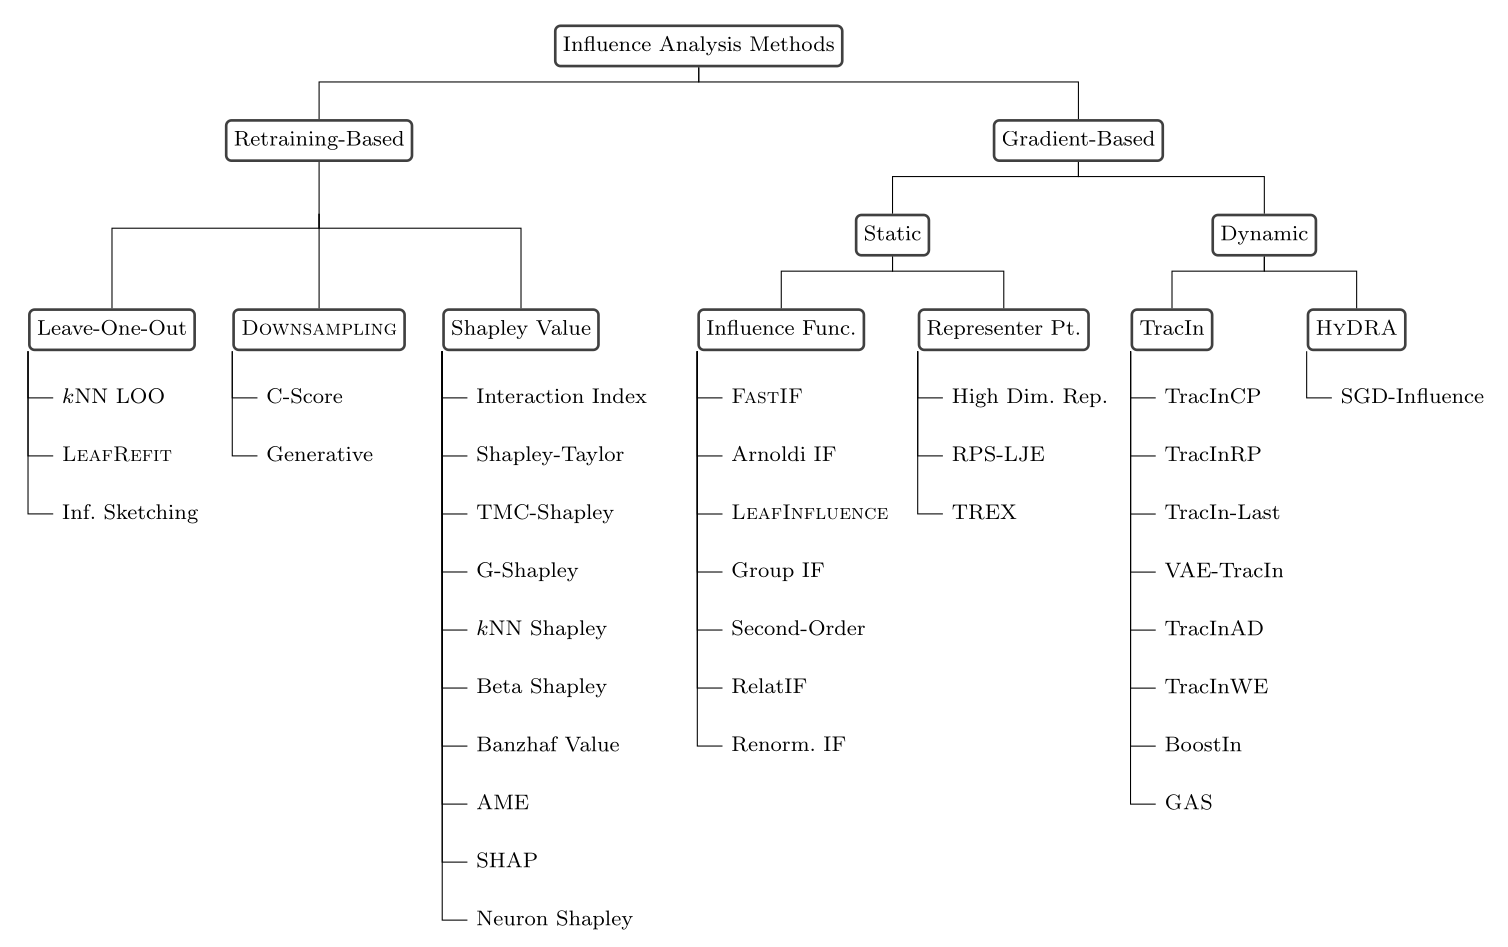
\includegraphics[width=1\textwidth]{figures/influence_analysis_methods.png}
    \caption{Categorization of different influence analysis methods and corresponding algorithms adopted from \cite{wang2024datashapleytrainingrun}}
    \fxnote{Design own image to match thesis style}
    \label{fig:influence_analysis_methods}
\end{figure}

\section{Paraphrased Corpora Analysis}
The authors of \cite{wang2024datashapleytrainingrun} did an experiment that is similar to the approach proposed in this article. There, the robustness of In-Run Data Shapley and influence functions is evaluated by identifying relevant individual corpora that have been paraphrased. They also calculate a rank based on the original training corpus and its paraphrased versions. For comparison, the BM25 \cite{bm25} distance is used as an oracle to assess the lexical similarity between the paraphrased versions and the original corpora, rather than the semantic similarity. Even with completely rewritten corpora, the corresponding original samples still rank very high according to In-Run Data Shapley and influence functions compared to BM25.
\\\\
\fxnote{Additional notes on related work (to be removed):}
\\\\
\fxnote{Further look into the paraphrased corpora analysis above to identify differences and similarities and elaborate an them.}
\\\\
\fxnote{Find related papers regarding layer selection/importance/influence with respect to predictions or explanations.}
\\\\
\fxnote{Also mention the pros of example based explanations: model-invariant as long as the model architecture uses gradients of a loss function based on inputs and outputs with respect to the input. Also, mention that the combination of gradient and example-based explanations does not require a retraining of the model.}
\\\\
\fxnote{Maybe write also about papers regarding LLMs (Attention, Transformer, ARLM vs. MLM), OLMo, Open-Instruct, Lima Dataset as well, since they are the basis of the experiments, etc.}
%\\\\
%\fxnote{Eventually include forward-, backward-pass, optimizers, etc.}

\section{Dimensionality and Performance}

\subsection{Traditional Dimensionality Reduction Techniques}
random projection

\subsection{Layer Selection}
\fxnote{introduce transformer architecture to establish connection to individual layers and gradient}

\subsubsection{Cornerstone Layers}
\cite{yeh2022betterlanguagedatainfluence}